% Created 2019-02-21 Thu 10:12
% Intended LaTeX compiler: pdflatex
\documentclass[15pt]{article}
\usepackage[utf8]{inputenc}
\usepackage[T1]{fontenc}
\usepackage{graphicx}
\usepackage{grffile}
\usepackage{longtable}
\usepackage{wrapfig}
\usepackage{rotating}
\usepackage[normalem]{ulem}
\usepackage{amsmath}
\usepackage{textcomp}
\usepackage{amssymb}
\usepackage{capt-of}
\usepackage{hyperref}
\usepackage{minted}
\usepackage[scaled]{helvet}
\renewcommand\familydefault{\sfdefault}
\usepackage[T1]{fontenc}
\usepackage{tabularx}
\usepackage[left=2cm, right=2cm,top=2cm]{geometry}
\author{Kevin Poli}
\date{\today}
\title{}
\hypersetup{
 pdfauthor={Kevin Poli},
 pdftitle={},
 pdfkeywords={},
 pdfsubject={},
 pdfcreator={Emacs 26.1 (Org mode 9.1.14)}, 
 pdflang={English}}
\begin{document}

\tableofcontents

\section{Telescope}
\label{sec:org8762791}
\begin{itemize}
\item Connor O’Hara: Image Processing (cohara1@stevens.edu)
\item Kevin Poli: Application/ Artist Tools Developer (kpoli@stevens.edu)
\item Philip Vitale: Application \& Systems Developer (pvitale@stevens.edu)
\item Brendan von Hofe: Machine Learning (bvonhofe@stevens.edu)
\end{itemize}
\subsection{Advisors:}
\label{sec:org9f083c0}
Hong Man (hman@stevens.edu), Jeff Thompson (JThomps4@stevens.edu)
\section{Intro}
\label{sec:org1a67f2f}
Telescope is a machine learning assisted toolkit for digital video compositors
with applications in visual effects, matte painting and diverse use cases
accross the video post production pipeline. Tools from existing compositing
packages will interact with a novel ML core to assist or completely automate the
rotoscoping process. Rotoscoping is the process of masking and segmenting
poritons of an image accross multiple moving frames, any feature length movie
will often consist of hundreds of rotoscoped shots with multiple tracked mattes
per image, and this is the primary job of thousands of roto artists accross the world.

We hope to make this process, fast, intuitive, and accesible to alleviate the
manual and time consuming process that makes up a huge chunk of the man hours
required to produce even low budget features. We believe that machine learning
is in the process of revolutionizing image processing, and that user driven
toolkits rather than black box command line workflows will bring our intelligent
core into the hands of the artists where they can thrive.
\subsection{Demonstration}
\label{sec:org09e13a6}
Rotoscoping is the process of frame by frame selecting and isolating a given feature (usually
an object or person) in a video, such that you can produce a video clip of
exclusively that selection on a transparent background

Lets walk through this step by step:

\begin{itemize}
\item First, our source image at frame 1, of Marceu the Mime
\begin{center}
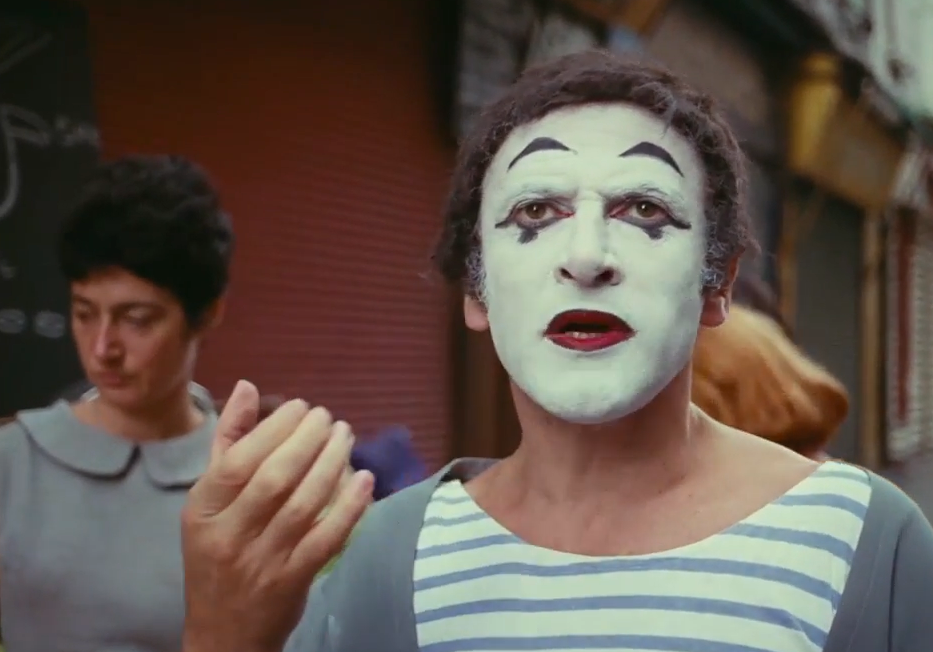
\includegraphics[width=.9\linewidth]{./roto/Capture.PNG}
\end{center}
\item Lets start by creating a selection just of the Mime's face and hand - these
are the features that are actually being "rotoscoped" out
\begin{center}
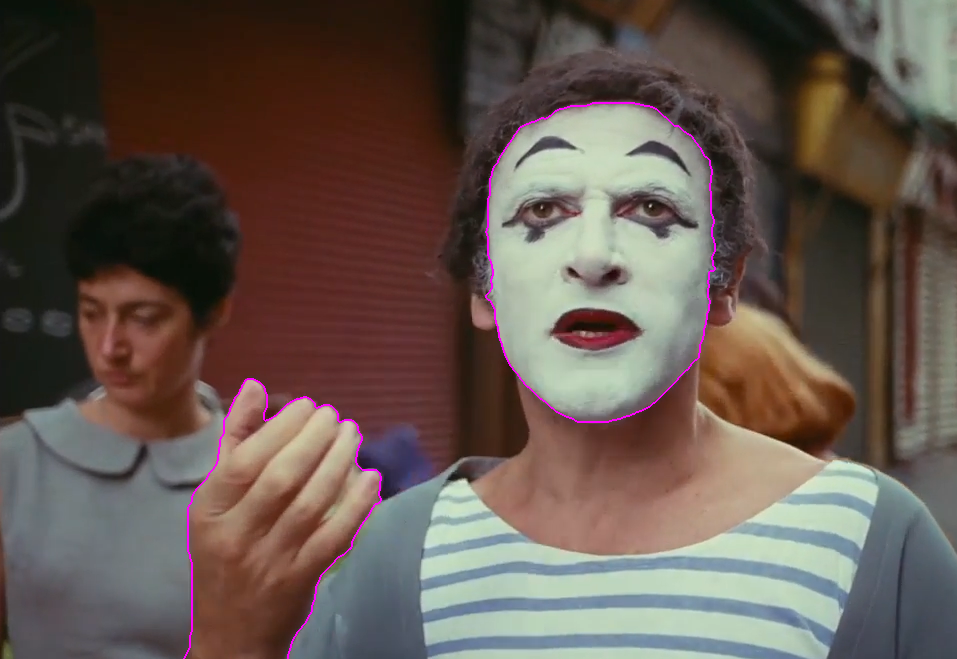
\includegraphics[width=.9\linewidth]{./roto/masked.PNG}
\end{center}
\item This purple selection represents a 'mask' which are the points and curves that
make up the boundary of what we are looking to isolate. Traditionally, artists
will digitally paint this selection in a software of their choice, by hand.
\item This selection or mask is different from a matte, which is another important
piece of terminology. A matte is a single channel image; meaning rather than
pixels having red,green,blue values, they only contain 1 value from 0-255
called 'alpha'. 'Alpha' will often be displayed in software as white. The
Matte of this selection is an image where only the pixels corresponding to the
selection are white, and all other pixels are black.
\begin{center}

\includegraphics[width=.9\linewidth]{./roto/matte.PNG}
\end{center}
\begin{itemize}
\item this is so that, under the hood, all we need to do is pixel-wise 'multiply' the
source image to the matte, meaning any pixels with a black 'zero value' in
the matte will become transparent, and any pixels in the white '255 value'
in the matte will remain.
\end{itemize}
\begin{center}
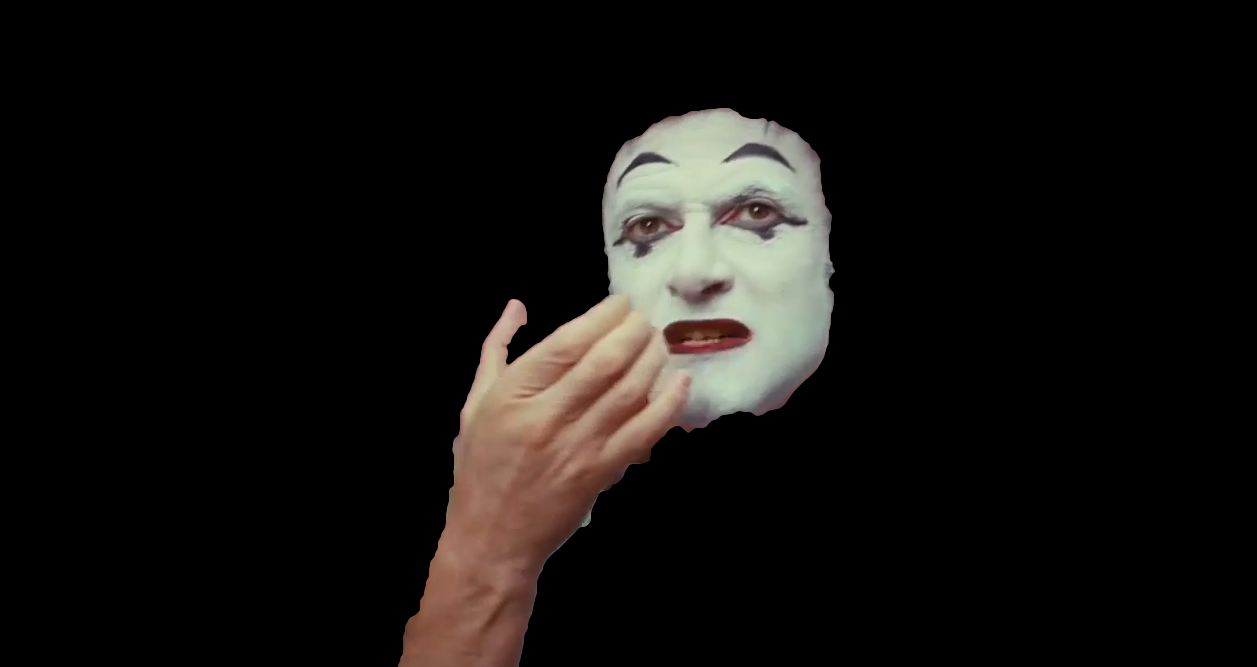
\includegraphics[width=.9\linewidth]{./roto/goals.PNG}
\end{center}
\begin{itemize}
\item Here is the result of that multiply, an image containing only the pixels we
selected before
\end{itemize}
\end{itemize}
\subsubsection{Frame By Frame}
\label{sec:org0397971}
Much of the challenge and tedium of rotoscoping comes from repeating the above
process for every frame, traditionally, artists will go frame by frame through
the video and manually adjust their selections to match the feature they are
isolating, here is the next frame of that video, with an adjusted selection for
clarity

\begin{center}
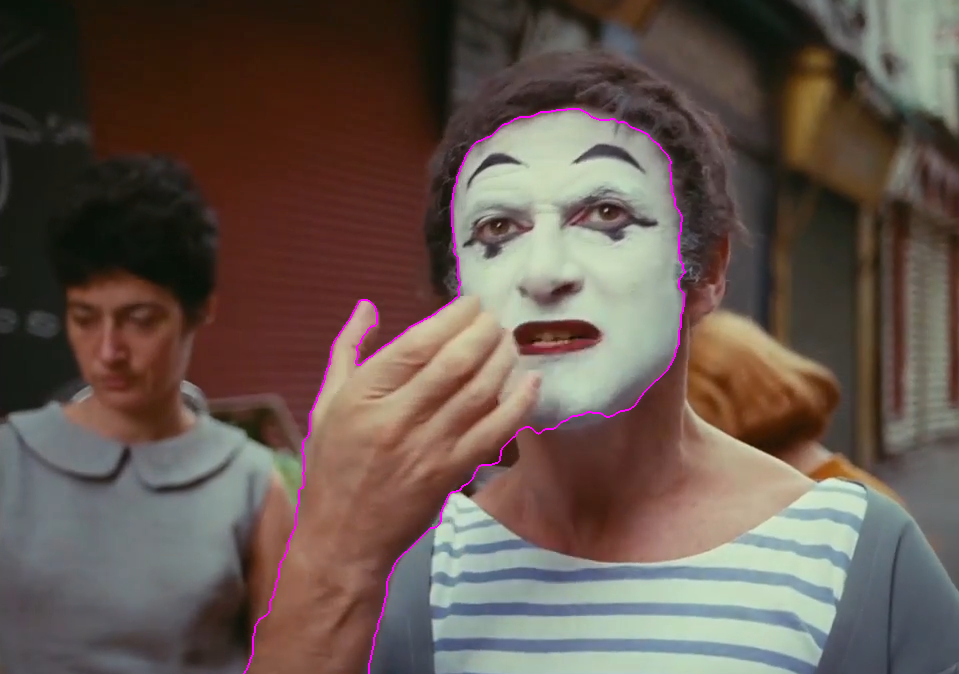
\includegraphics[width=.9\linewidth]{./roto/nextframe.PNG}
\end{center}

to see how the selections should move as features in the video move, check out
this gif that displays the matte on the left, with the source on the right, and
has selection lines on both
\url{https://www.google.com/url?sa=i\&rct=j\&q=\&esrc=s\&source=images\&cd=\&cad=rja\&uact=8\&ved=2ahUKEwj4poGei\_bdAhVvTt8KHYSXBs0QjRx6BAgBEAU\&url=https\%3A\%2F\%2Ftaukeke.com\%2F2014\%2F07\%2Frotoscoping-in-nuke\%2F\&psig=AOvVaw0rzB0nhBNxm\_0WD1VdybtL\&ust=1539062086451365}
\subsubsection{Use Cases}
\label{sec:orgc6d9392}
With our selection isolated, we can start to play with the image accordingly

By layering the source footage and our rotoscoped hand and face, we can apply an
effect, like the 'colorama' effect to only the pixels we roto'd previously

\begin{center}
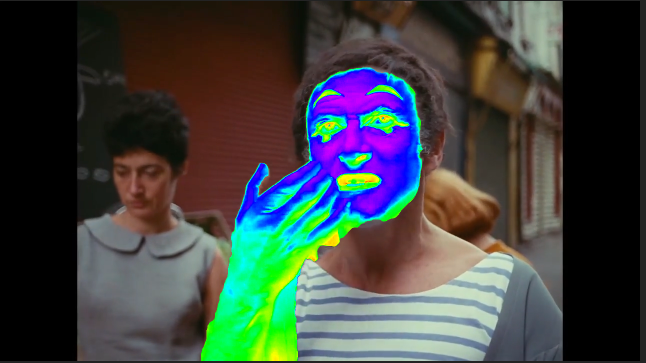
\includegraphics[width=.9\linewidth]{./roto/isolated.PNG}
\end{center}
\begin{enumerate}
\item Compositing
\label{sec:orge93f2f0}
The most popular use case for rotoscoping is Compositing, which is the process
of combining multiple images into one. Consider three layers to see how this is
done.

Say we want this red square video clip to appear 'behind' the Mime's face and
hand (note what appears black is acutally transparent)

\begin{center}

\includegraphics[width=.9\linewidth]{./roto/red.PNG}
\end{center}

We can grab our source clip and place the square image on top
  \begin{center}
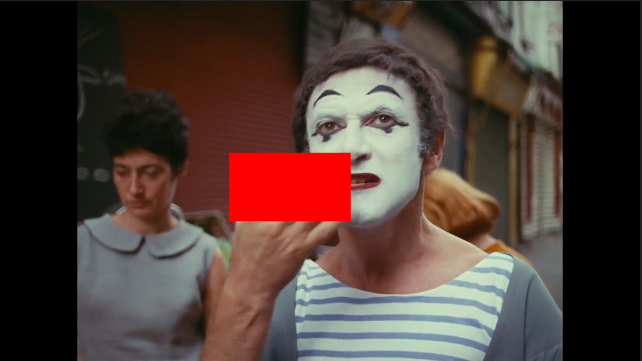
\includegraphics[width=.9\linewidth]{./roto/halfcomp.PNG}
\end{center}
Then grab our rotoscoped face and hand and place that on top
  \begin{center}
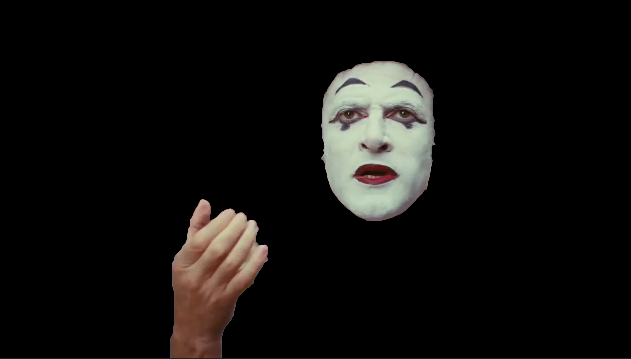
\includegraphics[width=.9\linewidth]{./roto/void.PNG}
\end{center}
and here is the desired effect

\begin{center}
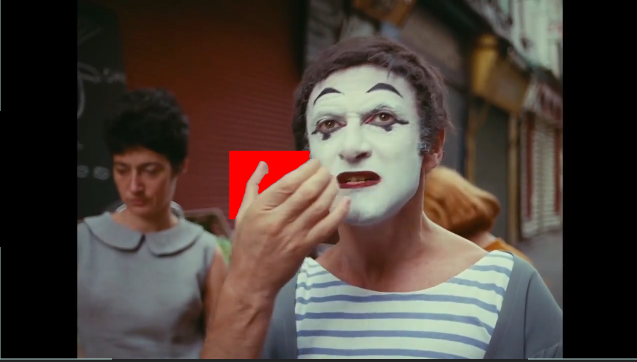
\includegraphics[width=.9\linewidth]{./roto/behind.PNG}
\end{center}
\end{enumerate}
\section{Technical Plan}
\label{sec:orgc4e4857}
\subsection{Components}
\label{sec:org12acc78}
Telescope as a product will consist of two primary modules, the Telescope Core,
which is a machine learning core assisted by traditional algorithmics that
implements the novel functionality of Telescope, and an exchange plugin that
allows existing professional compositing tools to interact with our proccesses.
Telescope For Nuke is our chosen example exhange plugin, designed to demonstrate
how the Telescope core can interact with existing artist workflows - but the
separation of core and plugin is designed such that Telescope can be implemented
into other software packages like Adobe After Effects or Blackmagic Design
Fusion at a later date.
\begin{center}
\begin{tabular}{ll}
Category & What are we using?\\
\hline
Communication & \\
Email & Gmail\\
Web Conferencing & Facebook Video\\
Instant Messaging & GroupMe\\
Collaboration & \\
Document Collaboration & Google Drive\\
File Sharing/Data Tracking & GitHub\\
Plugin Development & \\
OS Supported & Windows, Mac OS, Linux\\
Host Application & Nuke\\
Development Language & C++\\
Machine Learning Development & \\
Development Language & Python\\
Packages & PyTorch\\
\end{tabular}
\end{center}
\subsection{Algorithmics}
\label{sec:org6c7a857}

The algorithmic core of our plugin will take images (frames of videos) as input and output segmentation masks (mattes) as output. The goal of the masks is to identify all the discrete objects in the image. It is class-agnostic and therefore does not need to determine what the objects are (e.g. cat or dog) but rather the fact that they are discrete.
Our criteria for determining how well our model is accomplishing the task is the Intersection-over-Union metric (IoU). We have yet to determine what an acceptable IoU score is for industry applications.
The model will be a convolutional neural network. Specifically, we will begin with the UNet model (\url{https://arxiv.org/abs/1505.04597}). Initially, our primary dataset to train the model with will be the Panoptic Detection COCO dataset, modified for a class-agnostic task.
Further iterations of the model will take advantage of the additional information in EXR images to refine object mattes and the DAVIS video object segmentation dataset.

\subsection{Dependency Model}
\label{sec:org0969840}
\begin{center}
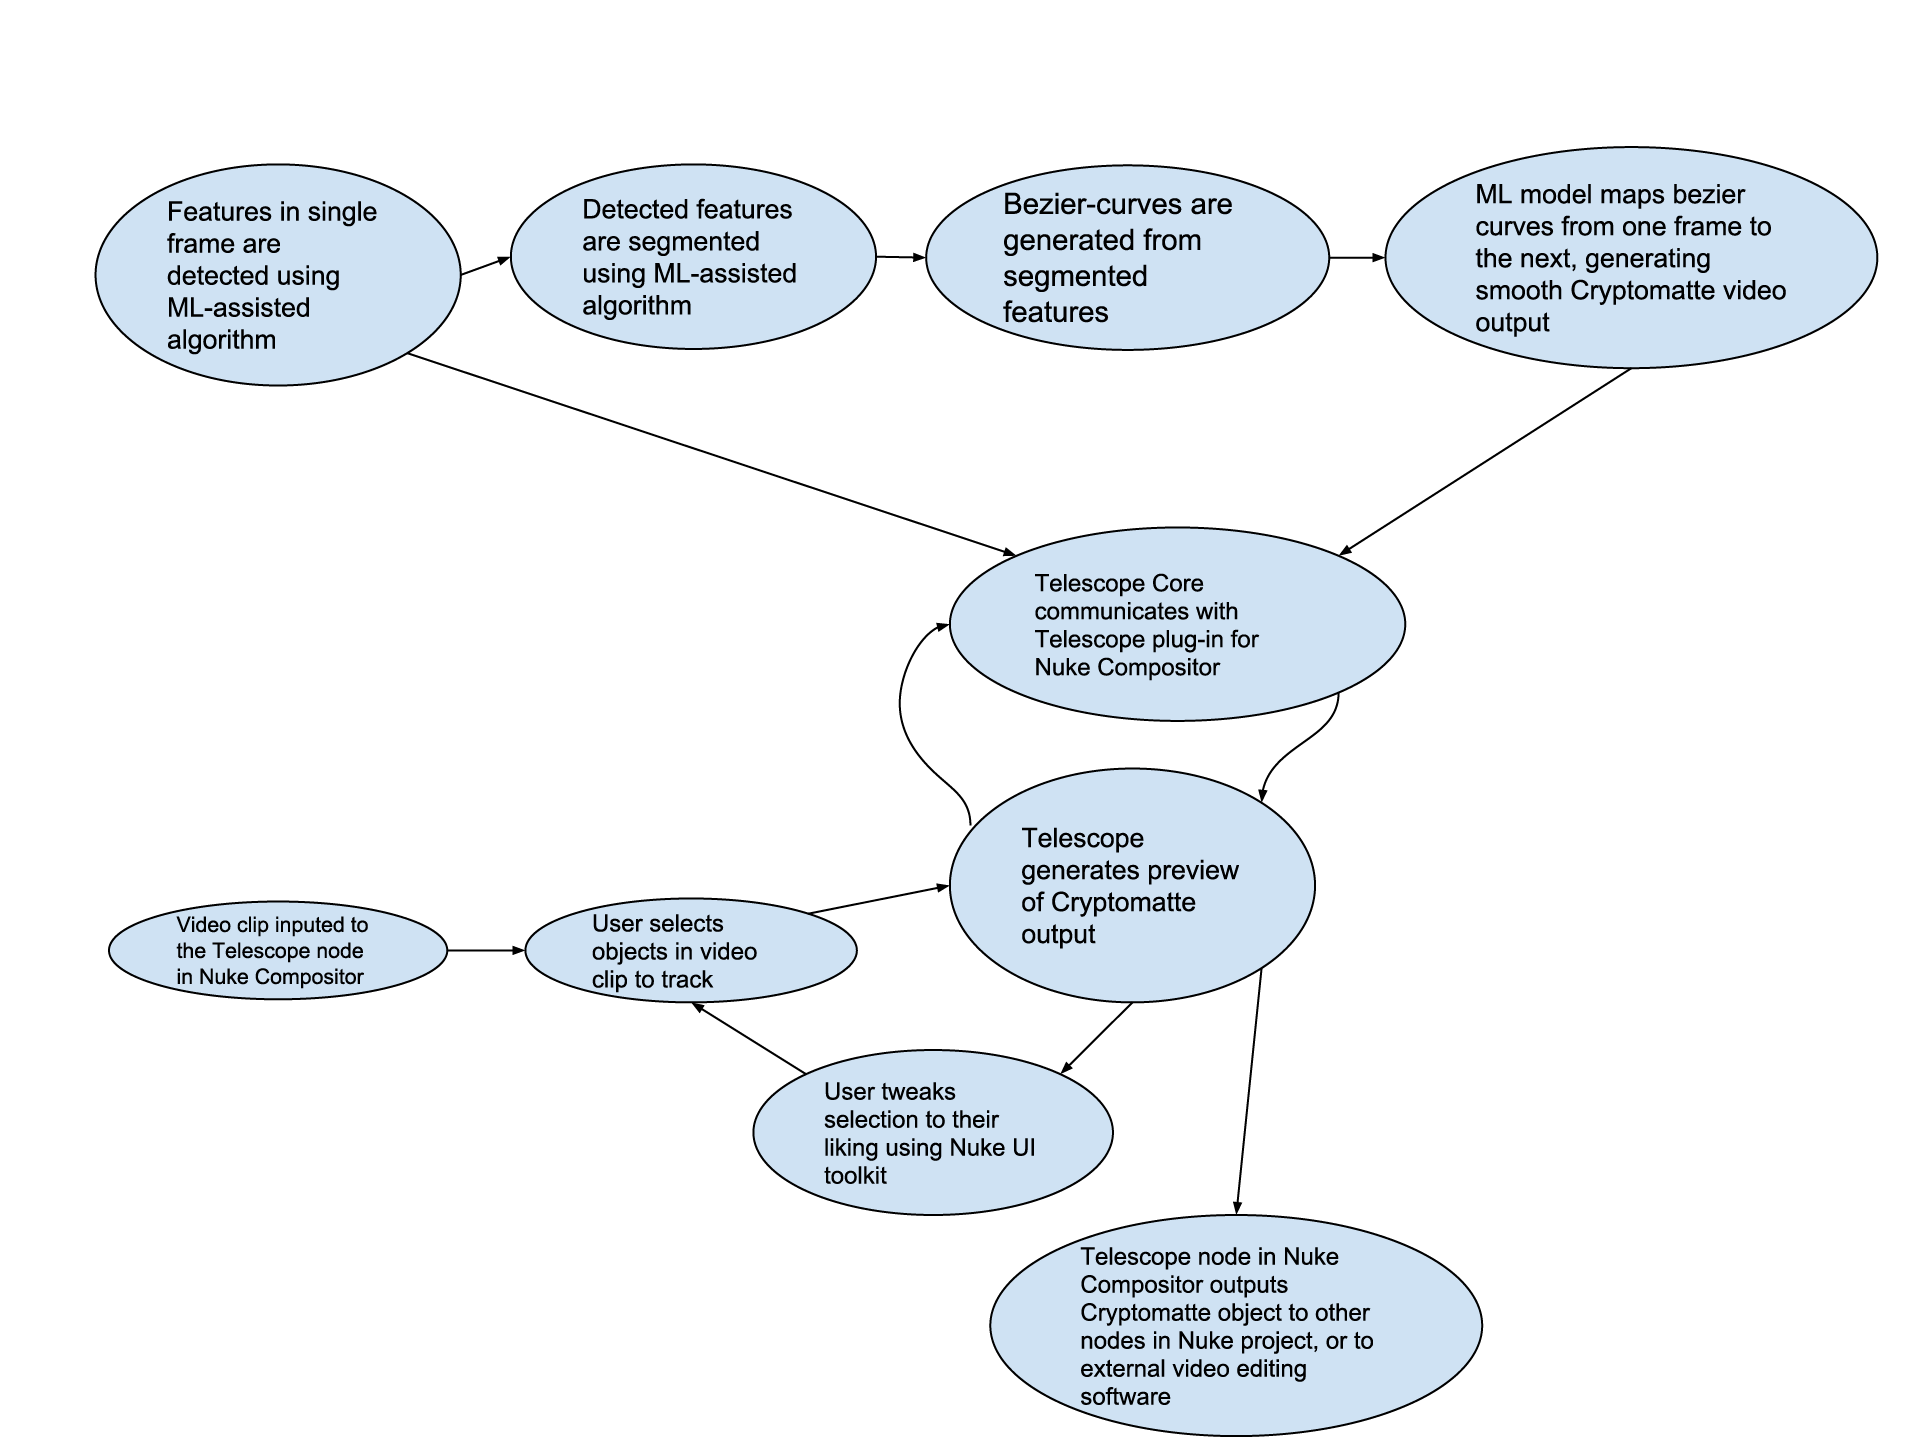
\includegraphics[width=18cm]{./Dgraph.pdf}
\end{center}
\subsection{Plugin UI Mockups}
\label{sec:orgc9bdd19}
\begin{center}
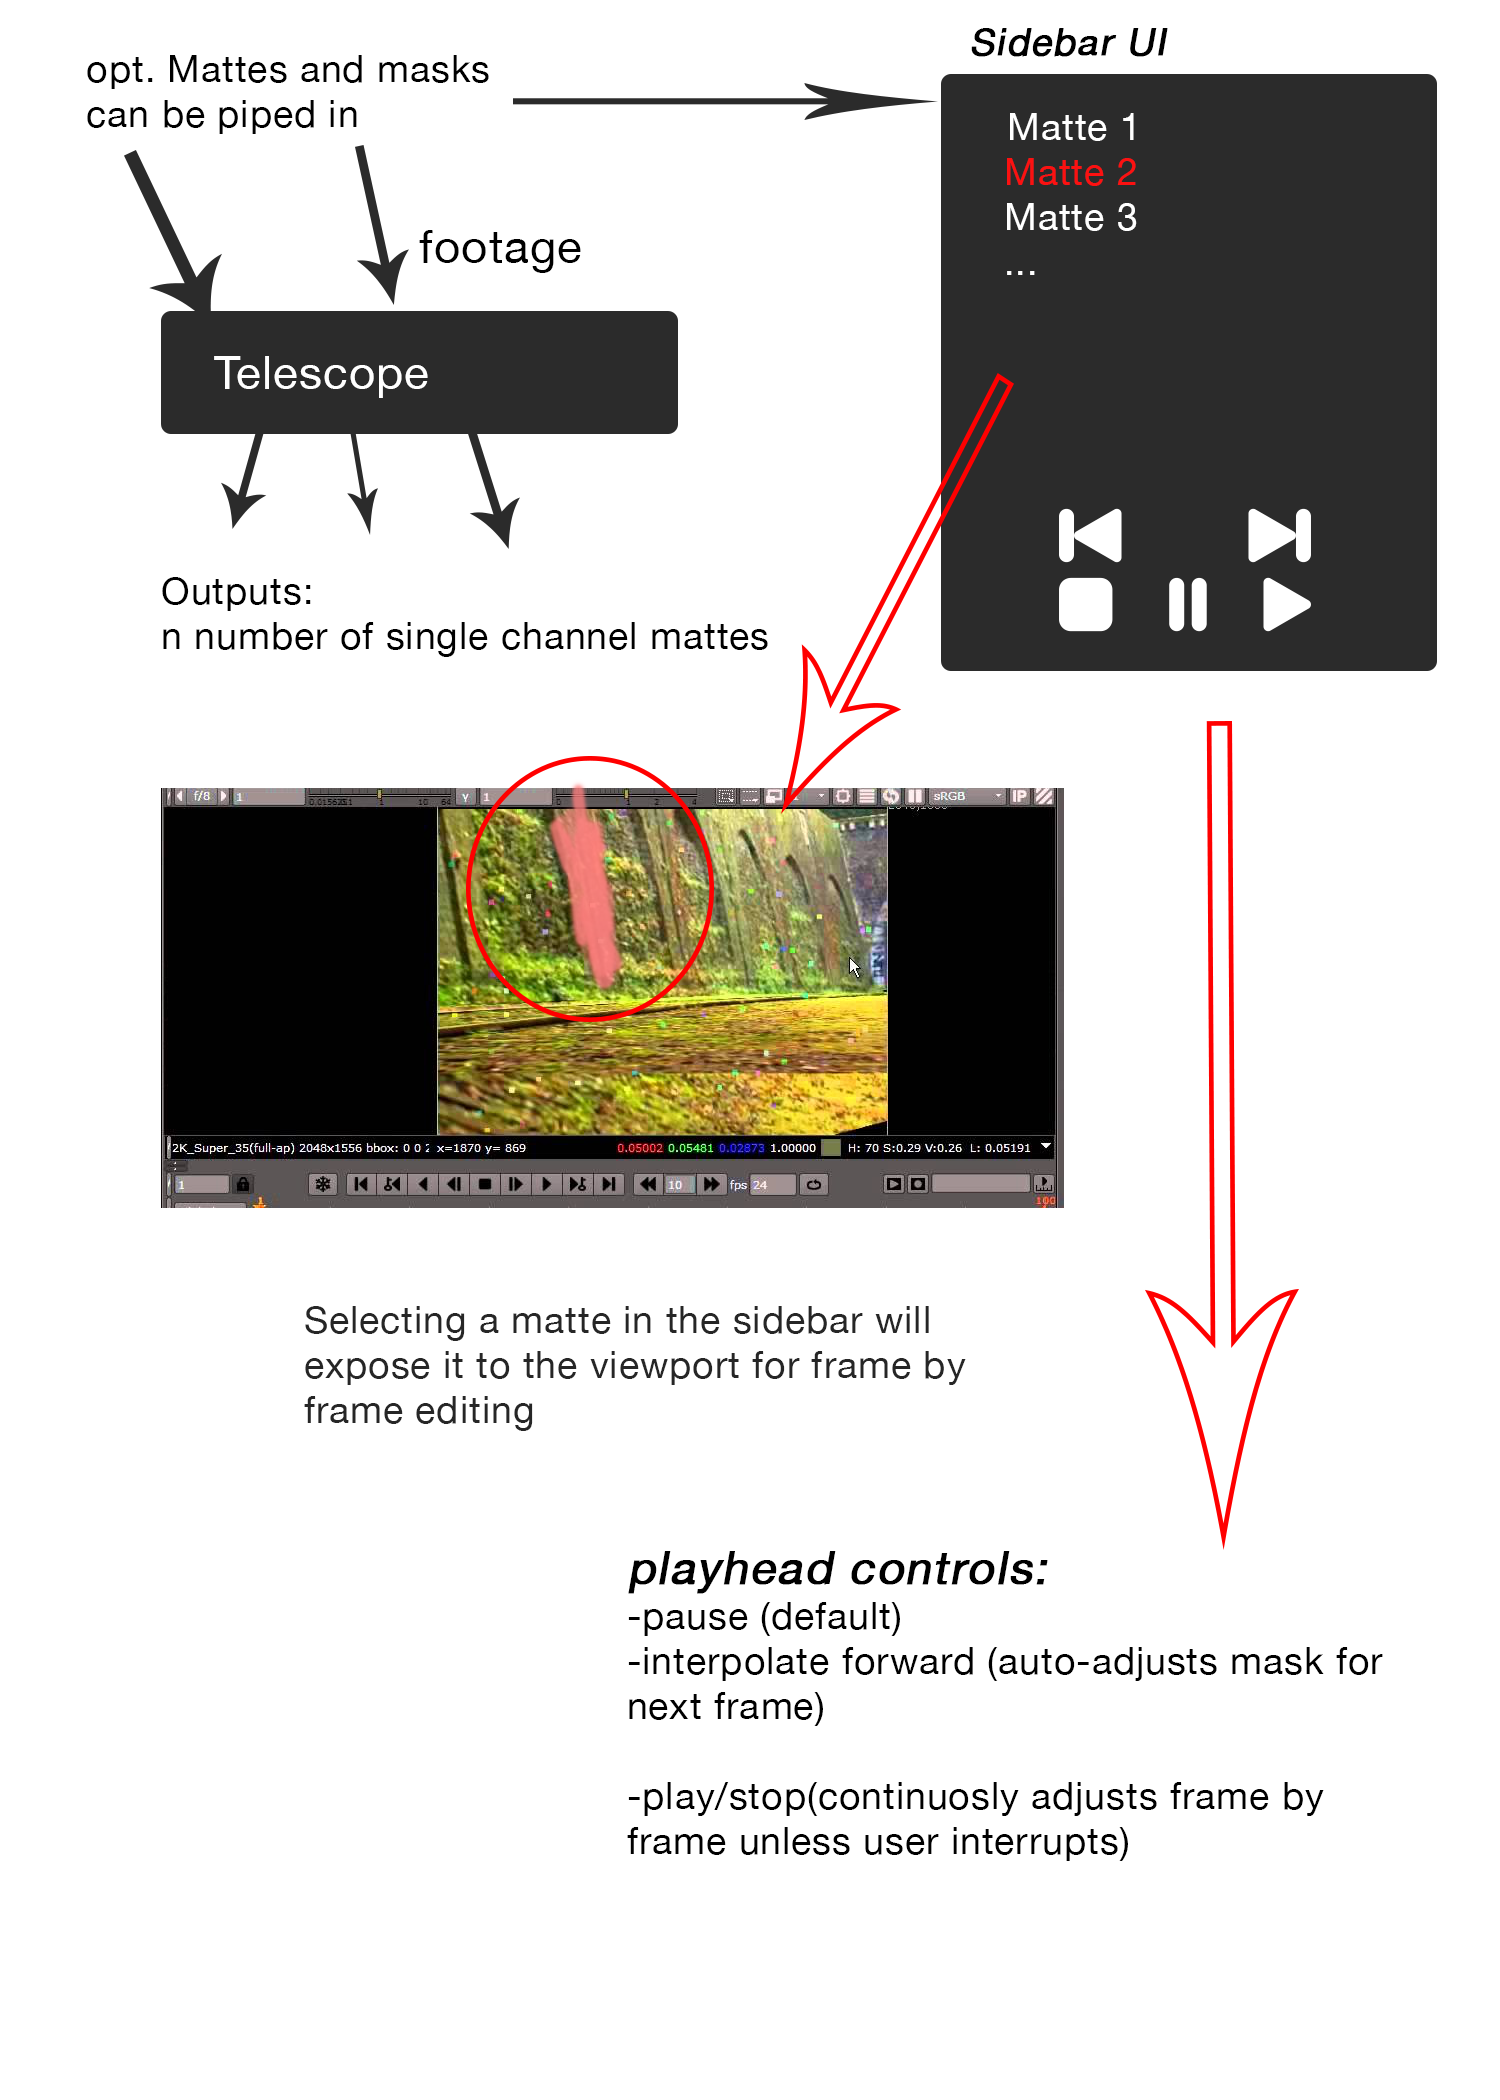
\includegraphics[width=.9\linewidth]{./mockup.png}
\end{center}
\subsection{Deep Learning Core}
\label{sec:org8395dbd}

\begin{center}
\includegraphics[width=.9\linewidth]{/Users/kevinpoli/org/.attach/image1_20181114_122910.png}
\end{center}
The core of our rotoscoping program is the deep learning model that takes the image to be cropped and an associated trimap as input (the two leftmost frames respectively), and outputs the cropped portion (rightmost frame). The image to be cropped can be of anything the user wishes. The associated trimap is used to identify the subject (foreground) in the image that the users wishes to crop out. It is drawn with auxiliary tools of our software to identify the definite foreground in white, the unsure foreground (e.g. hair) in grey, and definite background in black. The output is an alpha matte that can be used to crop the subject out of the original image.


\begin{center}
\includegraphics[width=.9\linewidth]{/Users/kevinpoli/org/.attach/image2_20181114_123001.png}
\end{center}
 The deep learning core is defined by the architecture (type of neural network) and its training process. The architecture is composed of two convolutional neural networks. The input data first passes through an encoder-decoder style network, commonly used for segmentation tasks (in the image above, the encoder is the first half of the ‘U’ and the decoder is the second half). Through the successive steps of the network, the image is transformed into different representations called feature maps. The initial representation is the input image itself along with the trimap. As a multidimensional array it has a shape of [height, width, channels]. In this case, there are 4 channels. Three are the RGB channels of the input image, and the last is the associated trimap. As the image passes through the encoder, the feature map representing the image becomes shorter and thinner, but much deeper (e.g. shape of [7, 7, 2048]. The receptive field[1] of the convolutions grows, theoretically allowing it to make higher level abstractions about the subject matter of the image. The decoder then uses this information to eventually generate a single channel image with the same height and width of the original as it uses transposed convolutions.
        The second convolutional neural network is much simpler, composed of only a couple convolutional layers similar to the first of the encoder’s. The input to this network is the original image along with the alpha matte produced from the first network. It outputs a refined version of the alpha matte.
        The training process involves feeding the networks images that we also have ground truth alpha mattes for. After the network outputs a prediction for the alpha matte, we compare it with the ground truth alpha matte using a loss function. This loss function is a combination of two loss functions, the alpha prediction loss, and the compositional loss. The former simply calculates the pixel-wise squared error between mattes. The latter does the same calculation but with the original RGB image composited with the ground truth and predicted alpha mattes. Because of the differentiable nature of the loss functions and backpropagation[2], the weights of the neural network are able to be updated to perform the associated task of rotoscoping slightly better after training on each image. We repeatedly train on the entire dataset until improvements become negligible.
\subsubsection{More Information}
\label{sec:org4c4644b}
\begin{itemize}
\item \url{https://medium.com/mlreview/a-guide-to-receptive-field-arithmetic-for-convolutional-neural-networks-e0f514068807}
\item \url{https://medium.com/datathings/neural-networks-and-backpropagation-explained-in-a-simple-way-f540a3611f5e}
\end{itemize}
\subsection{Completion Schedule}
\label{sec:org6ca1953}
As the models have taken to exceptionally long training times, we have pivoted
slightly to the goal of having single frame at a time calculated at every frame
via the plugin utilizing the ML core. This is in contrast to our previous goal
which would use motion within the image as part of the ML core. These features
may still come to the plugin, but it is likely that they will arrive as
traditionally algorithmic and not ML based features, as there are already algorithmic techniques for
making mattes and trimaps more consistent across frames.
\begin{center}
\begin{tabularx}{\textwidth}{XXl}
Applications & Machine Learning & Week\\
\hline
\sout{Integrate ML Module Loader into existing plugin Node} & \sout{Explore new training schedules and perform hyperparameter tuning} & 2/14/\\
\hline
Test ML Module Loader on Various Models & \sout{Continued refinement on the single frame model} & 2/21/\\
\hline
\sout{Research Image Interpolation} & Research into multi-resolution support & 2/27/\\
\hline
\sout{Test interpolations} & continued research into resolution independence & 3/7/\\
\hline
\sout{Begin integrating interpolation tools} & Begin implementing resolution independence & 3/14/\\
\hline
Refine interpolation tools & Research ML based frame Interpolation & 3/21/\\
\hline
Research any additional artist tools required & Research additional ML artist tools & 3/28/\\
\hline
implement additional convenience tools if necessary & implement ML frame interpolation and tools if necessary & 4/4/\\
\hline
continued refinement & continued refinement & 4/11/\\
\end{tabularx}
\end{center}


\section{Team}
\label{sec:orgfe8ede7}
\subsection{Roles}
\label{sec:org70817ae}
\begin{itemize}
\item Connor O’Hara: Image Processing (cohara1@stevens.edu)
\item Kevin Poli: Application/ Artist Tools Developer (kpoli@stevens.edu)
\item Philip Vitale: Application \& Systems Developer (pvitale@stevens.edu)
\item Brendan von Hofe: Machine Learning (bvonhofe@stevens.edu)
\end{itemize}



\subsection{Delegation of Tasks}
\label{sec:orgfbfdd38}

\subsubsection{Connor O’Hara}
\label{sec:org1eb55be}
\begin{enumerate}
\item Last Week
\label{sec:org5d047d0}
\begin{itemize}
\item worked on getting GPU resources
\end{itemize}
\item Update
\label{sec:orgb027c37}
\begin{itemize}
\item meeting hopefully on friday, still in the works. Also began experimentation with trained ML models.
\end{itemize}
\item For Next week
\label{sec:orga30c227}
\begin{itemize}
\item revisit getting GPU resources from art department and continue research into the ML model.
\end{itemize}
\end{enumerate}

\subsubsection{Kevin Poli}
\label{sec:org25f3f9a}
\begin{enumerate}
\item Last Week
\label{sec:org3e92556}
\begin{itemize}
\item Resuming work in Nuke, and exploring API for novel interactions
\end{itemize}
\item Update
\label{sec:org9450e9e}
\begin{itemize}
\item Functional 1-channel 3 color drawing node for TriMaps
\end{itemize}
\item For Next Week
\label{sec:org8f0ba34}
\begin{itemize}
\item implement more control over dialations (inside, outside, centering)
\end{itemize}
\end{enumerate}
\subsubsection{Phil Vitale}
\label{sec:org0bece8b}
\begin{enumerate}
\item Last Week
\label{sec:org6286cf2}
\begin{itemize}
\item rough draft of the module loader, may be as simple as shellscript/watch folders
\end{itemize}

\item Update
\label{sec:orgd2dea7e}
\begin{itemize}
\item work on module loader continues, investigation into calling python scripting
from C++ NDK is promising.
\end{itemize}
\item For Next Week
\label{sec:org842bf87}
\begin{itemize}
\item functional module loader, no shellscript/watch folders
\end{itemize}
\end{enumerate}
\subsubsection{Brendan Von Hofe}
\label{sec:orgcf2c0b9}
\begin{enumerate}
\item Last Week
\label{sec:orgd9db3d5}
\begin{itemize}
\item Fine-tune the model and optimize hyperparameters for better quality outputs.
\end{itemize}
\item Update
\label{sec:org529ea85}
\begin{itemize}
\item Re-organized the code, wrote build scripts, etc. to allow for easy experimentation on various machines. Logging has also been improved to thoroughly report on results from experiments.
\end{itemize}
\item For Next Week
\label{sec:org6f04037}
\begin{itemize}
\item Begin testing on cloud and read research papers to illuminate potential areas of improvement. \url{https://arxiv.org/pdf/1707.08289v1.pdf}
\end{itemize}
\end{enumerate}
\end{document}
